Keberhasilan mencapai tujuan dan peningkatan minimum clearance yang telah
dibahas pada Subbab~\ref{sec:keberhasilan_tabrakan} dan
Subbab~\ref{sec:analisis_keselamatan} belum cukup menggambarkan kualitas
navigasi secara menyeluruh, karena keduanya tidak menangkap bagaimana
\textit{proses} robot bergerak menuju tujuan tersebut. Gerakan yang terlalu
berosilasi, meskipun pada akhirnya berhasil dan tetap aman, dapat
mengurangi efisiensi operasional dan kenyamanan pengamatan, serta secara
teoritis merupakan kelemahan yang melekat pada \textit{Artificial Potential
Field} (APF) di sekitar \textit{obstacle} pada lorong sempit atau
\textit{local minima}, sebagaimana telah dibahas pada
Subbab~\ref{sec:algoritma_navigasi}. APFPlanner pada penelitian ini
sebenarnya telah dilengkapi mekanisme deteksi osilasi berbasis kesamaan
arah gaya antar-siklus (Persamaan~\ref{eq:osc_detect}) yang aktif pada
\textit{kedua} konfigurasi, karena merupakan bagian dari perencana inti,
bukan bagian dari adaptasi fuzzy. Subbab ini mengevaluasi apakah adaptasi
fuzzy memberikan kontribusi tambahan terhadap kestabilan gerak di atas
mekanisme dasar tersebut, atau justru tidak memberikan perbedaan yang
berarti pada beberapa kondisi lingkungan.

\subsection{Definisi Smoothness yang Digunakan}

Penelusuran terhadap \texttt{experiment\_logger.py}, \texttt{analyze\_results.py},
\texttt{plot\_trajectories.py}, dan \texttt{Plot\_trajectories\_dynamic.py}
pada implementasi aktual menunjukkan bahwa metrik \textit{smoothness} secara
eksplisit, baik berbasis perubahan \textit{heading} maupun kelengkungan
lintasan, \textbf{tidak dihitung} pada pipeline penelitian ini. Sebagai
penggantinya, subbab ini menggunakan dua sumber bukti yang telah tersedia.
Pertama, kecepatan angular rata-rata (\texttt{avg\_angular\_vel}) yang telah
didefinisikan pada Persamaan~\ref{eq:avg_vel} (Subbab~\ref{sec:metrik})
digunakan sebagai proksi kuantitatif, karena secara matematis berkaitan
langsung dengan laju perubahan \textit{heading} robot meskipun bukan
\textit{smoothness score} yang didefinisikan secara terpisah. Kedua,
analisis visual terhadap trajektori aktual digunakan sebagai bukti
kualitatif pelengkap untuk menilai bentuk lintasan dan konsistensi
antar-\textit{trial}, mengikuti pendekatan yang telah diterapkan pada
penelitian navigasi berbasis APF lainnya yang juga mengandalkan inspeksi
visual lintasan ketika metrik kehalusan terstandardisasi tidak
tersedia~\cite{Lv2024}.

\begin{table}[H]
\centering
\caption{Perbandingan kecepatan angular rata-rata antara konfigurasi
\textit{baseline} dan \textit{proposed method} pada keempat pasangan
skenario.}
\label{tab:angvel_deskriptif}
\begin{tabular}{lccc}
\toprule
\textbf{Pasangan} & \textbf{Baseline $\omega$ (rad/s)} & \textbf{Proposed $\omega$ (rad/s)} & \textbf{$\Delta$ (\%)} \\
\midrule
S1--S5 & 0,091 $\pm$ 0,002 & 0,083 $\pm$ 0,001 & -8,8 \\
S2--S6 & 0,134 $\pm$ 0,046 & 0,103 $\pm$ 0,001 & -23,1 \\
S3--S7 & 0,167 $\pm$ 0,002 & 0,188 $\pm$ 0,015 & +12,6 \\
S4--S8 & 0,130 $\pm$ 0,022 & 0,133 $\pm$ 0,019 & +2,3 \\
\bottomrule
\end{tabular}
\end{table}

\subsection{Analisis Kualitatif Lintasan per Pasangan}

\begin{figure}[H]
\centering
\begin{subfigure}[t]{0.48\textwidth}
\centering
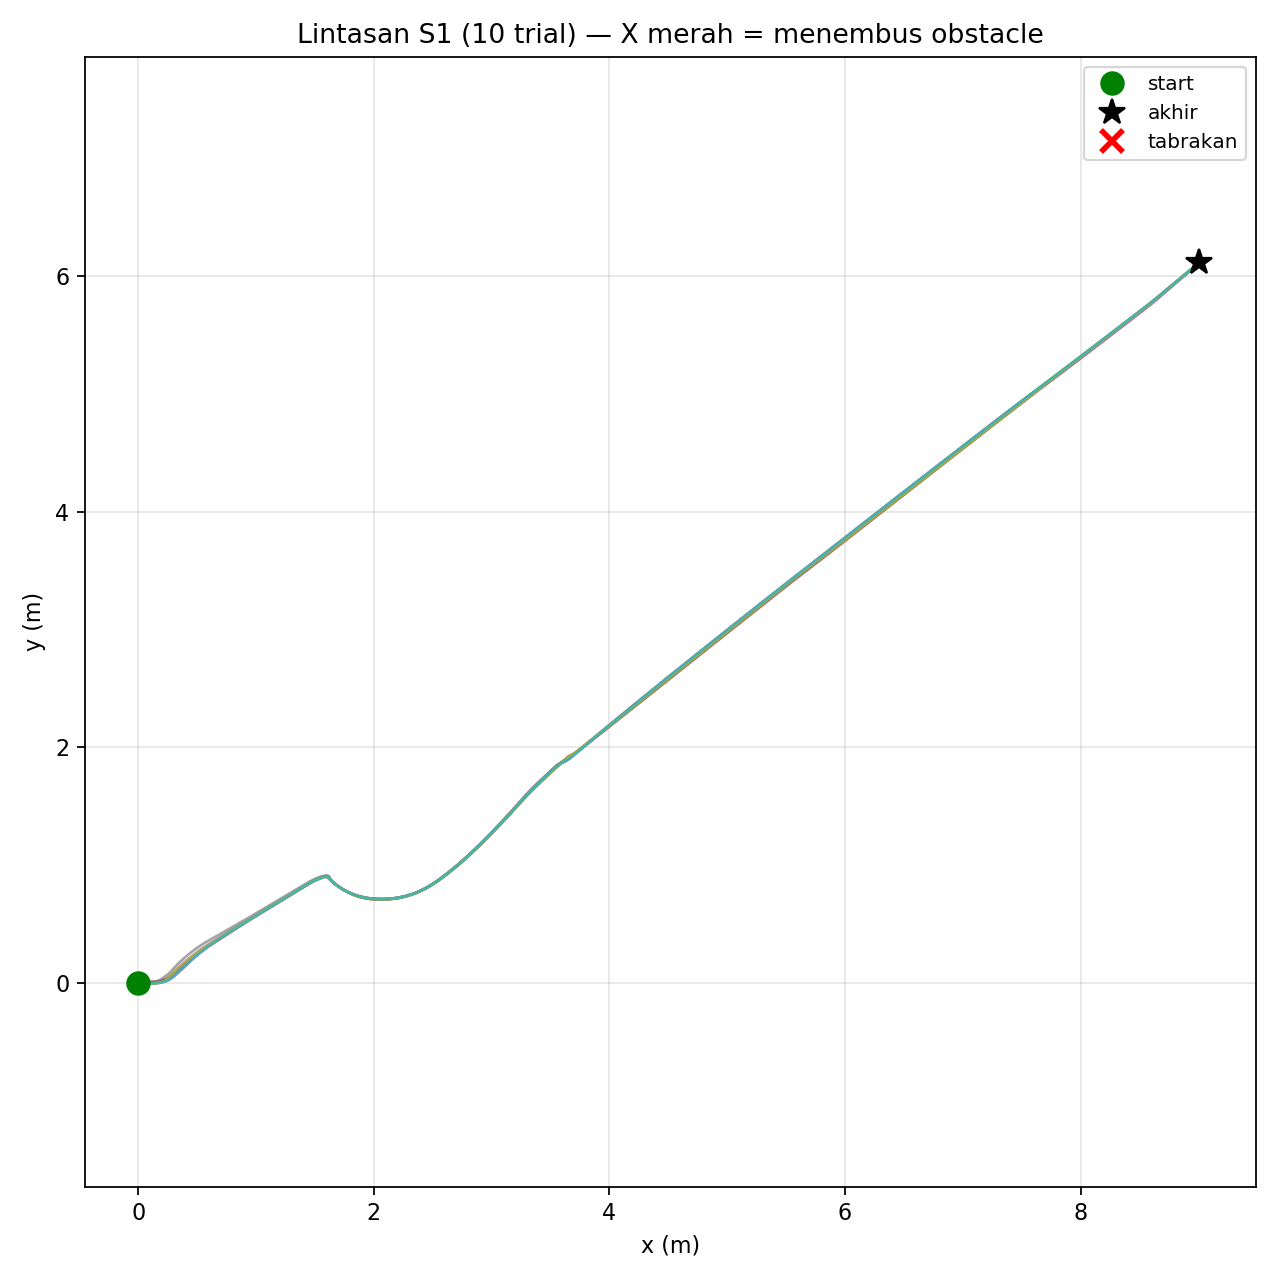
\includegraphics[width=\textwidth]{gambar/4.6_traj_S1.png}
\caption{S1 (baseline)}
\end{subfigure}
\hfill
\begin{subfigure}[t]{0.48\textwidth}
\centering
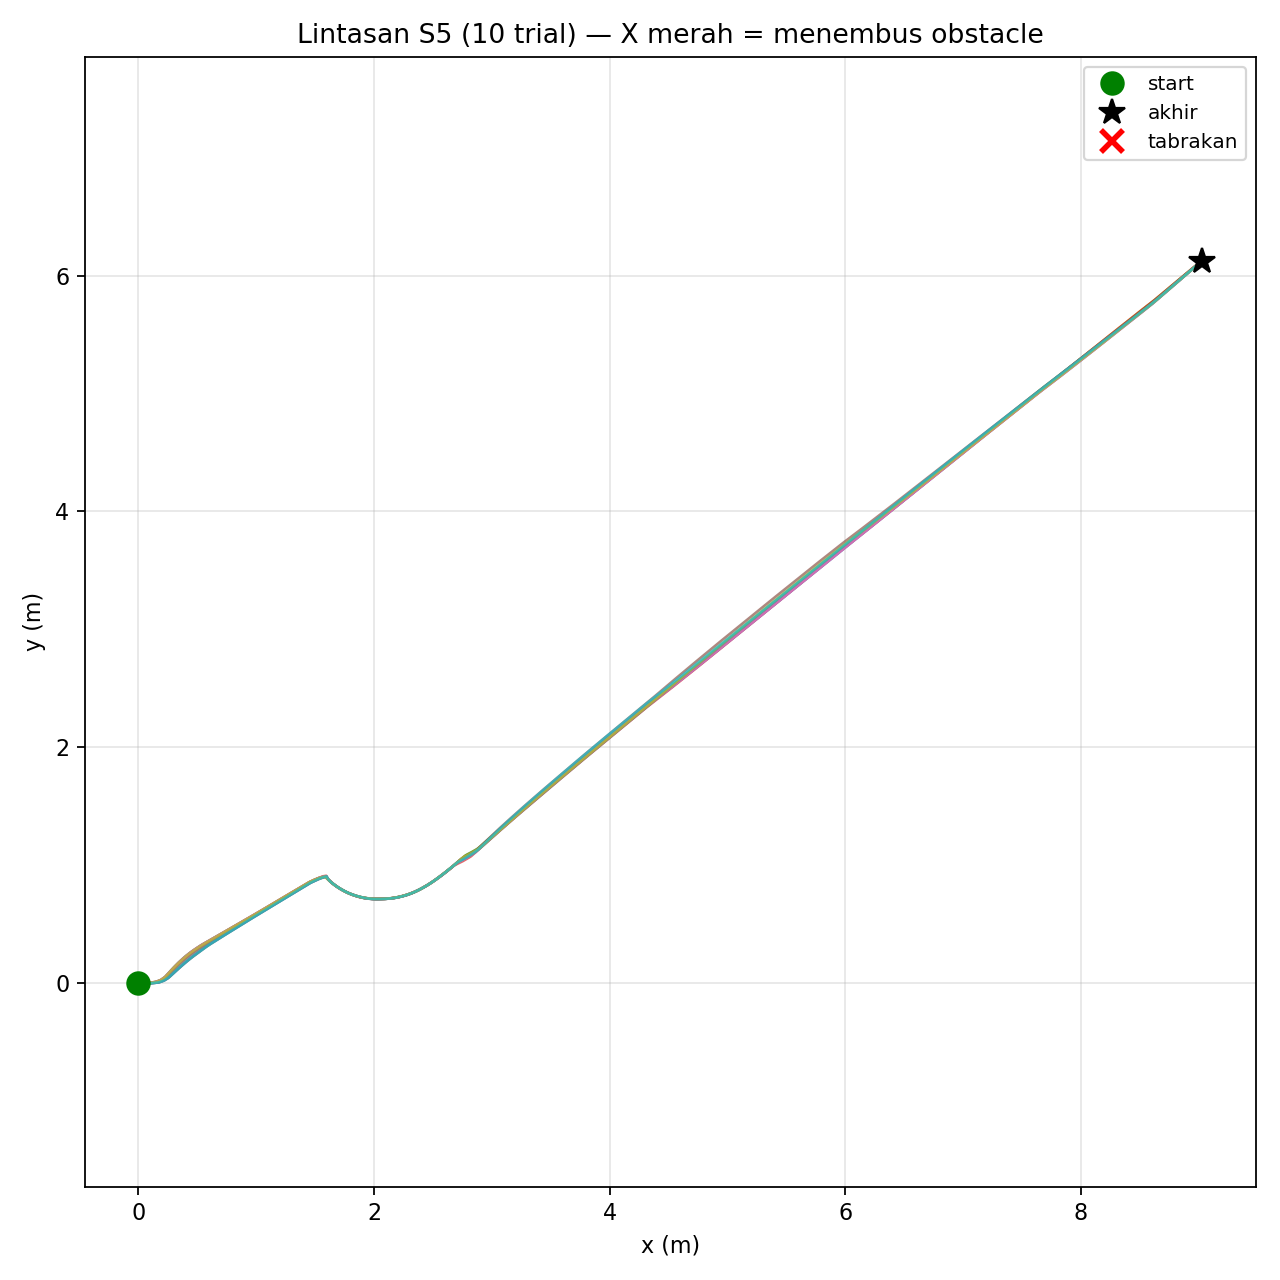
\includegraphics[width=\textwidth]{gambar/4.6_traj_S5.png}
\caption{S5 (proposed)}
\end{subfigure}
\caption{Lintasan S1 (kiri) dan S5 (kanan), lingkungan terbuka tanpa
\textit{obstacle}.}
\label{fig:traj_s1s5}
\end{figure}

Pada pasangan S1/S5 (Gambar~\ref{fig:traj_s1s5}), kedua konfigurasi
menghasilkan bentuk lintasan yang praktis identik, termasuk lekukan kecil
yang sama di sekitar $x=1,5$~m pada kesepuluh \textit{trial} di masing-masing
konfigurasi. Hal ini wajar mengingat tidak ada \textit{obstacle} aktif yang
perlu direspons pada skenario ini, sehingga tidak terdapat perbedaan
kualitatif yang dapat dilaporkan secara jujur pada pasangan ini.

\begin{figure}[H]
\centering
\begin{subfigure}[t]{0.48\textwidth}
\centering
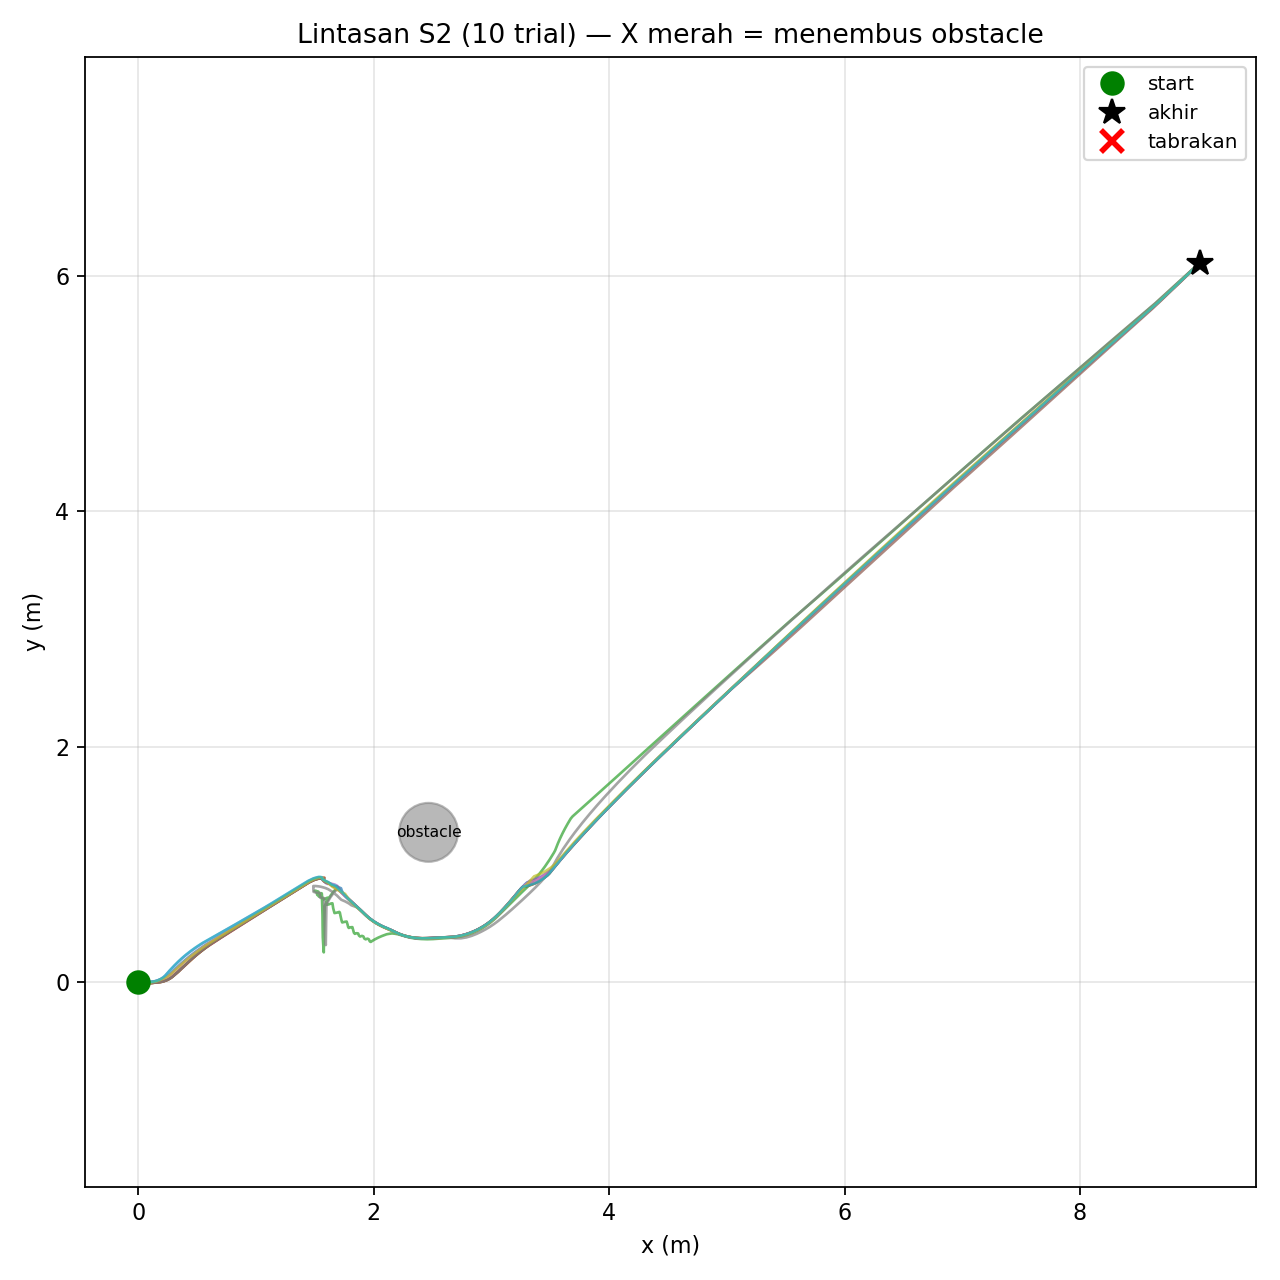
\includegraphics[width=\textwidth]{gambar/4.6_traj_S2.png}
\caption{S2 (baseline)}
\end{subfigure}
\hfill
\begin{subfigure}[t]{0.48\textwidth}
\centering
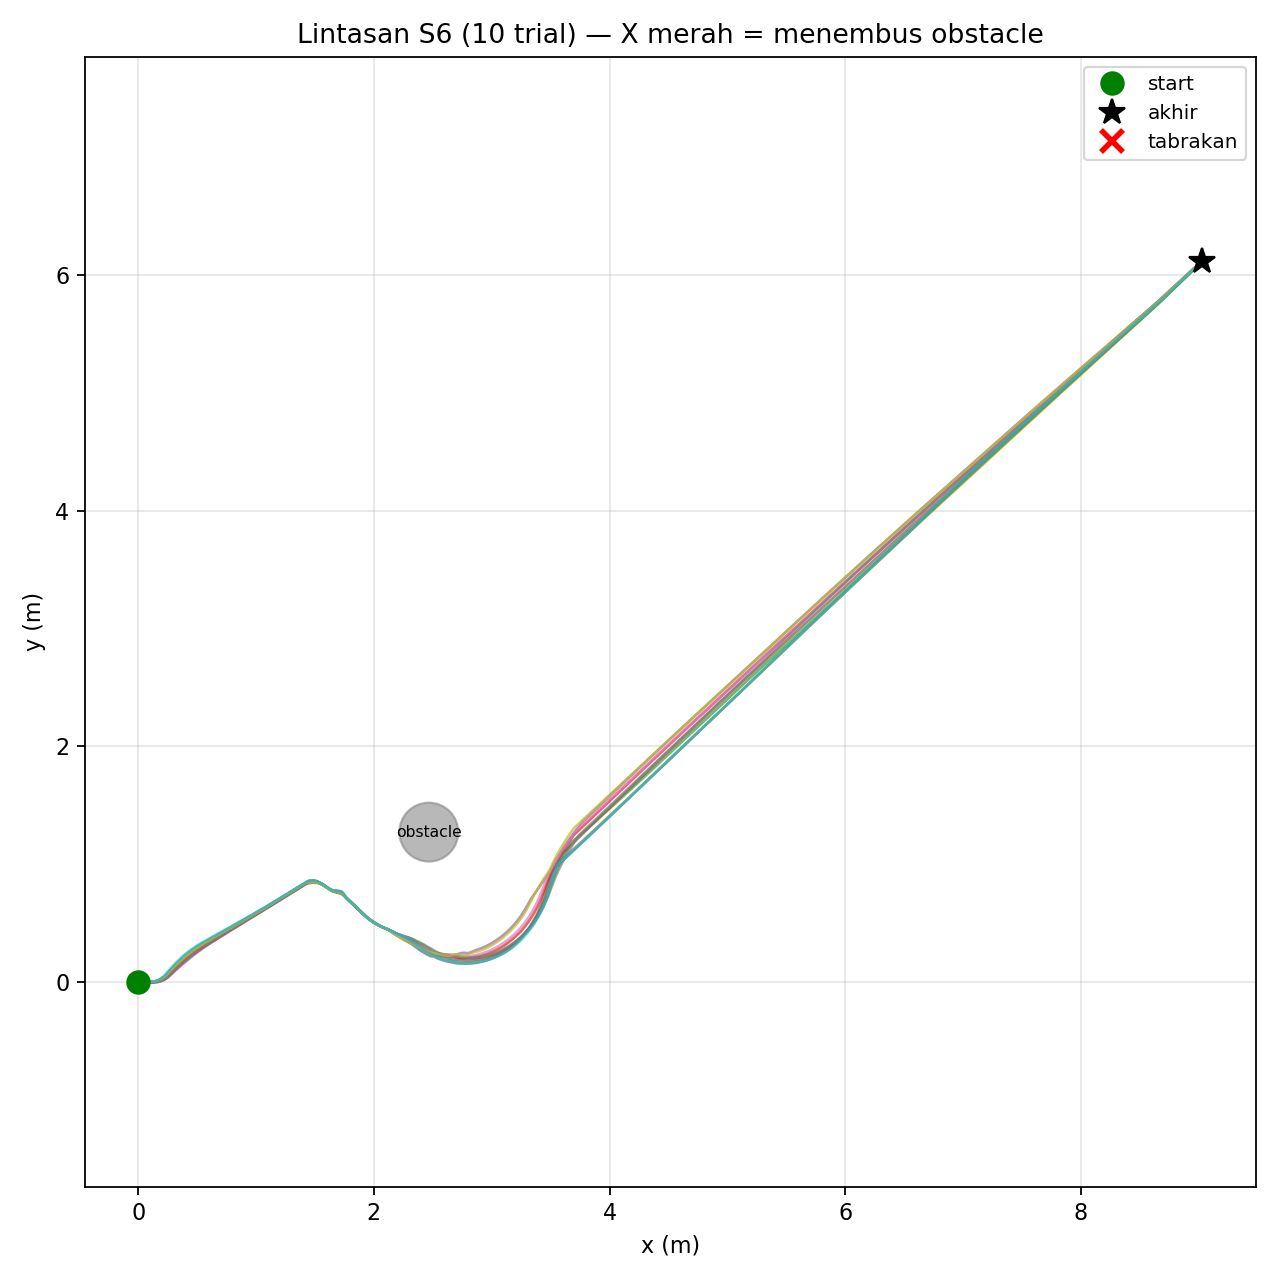
\includegraphics[width=\textwidth]{gambar/4.6_traj_S6.png}
\caption{S6 (proposed)}
\end{subfigure}
\caption{Lintasan S2 (kiri) dan S6 (kanan), lingkungan dengan satu
\textit{obstacle} statis.}
\label{fig:traj_s2s6}
\end{figure}

Pada pasangan S2/S6 (Gambar~\ref{fig:traj_s2s6}), satu dari sepuluh
\textit{trial} \textit{baseline} (S2) menunjukkan koreksi arah mendadak
berupa pola zig-zag tajam tepat saat melewati \textit{obstacle}, sementara
seluruh sepuluh \textit{trial} \textit{proposed method} (S6) konsisten
menghasilkan kurva yang mulus tanpa pola serupa. Temuan ini konsisten
dengan standar deviasi kecepatan angular S2 yang relatif tinggi
($\pm$0,046~rad/s) dibandingkan S6 yang jauh lebih konsisten
($\pm$0,001~rad/s) pada Tabel~\ref{tab:angvel_deskriptif}, mengindikasikan
bahwa variasi tersebut didorong oleh satu \textit{trial} yang menyimpang
dari pola umum, bukan ketidakstabilan yang merata pada seluruh
\textit{trial baseline}.

\begin{figure}[H]
\centering
\begin{subfigure}[t]{0.48\textwidth}
\centering
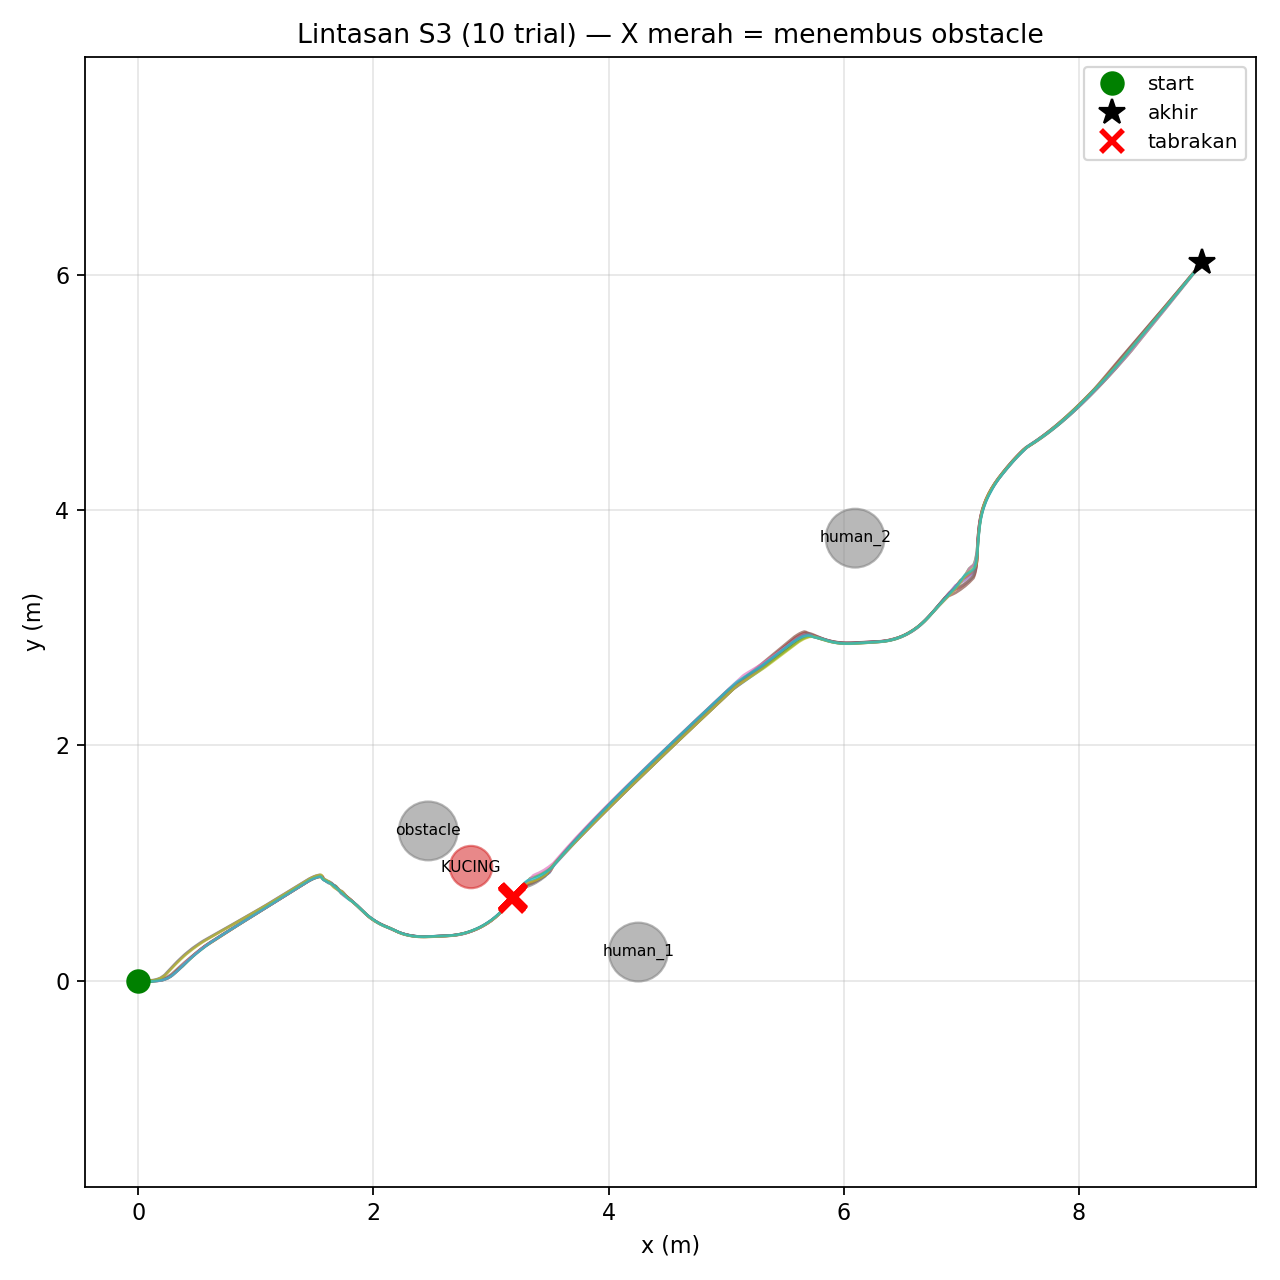
\includegraphics[width=\textwidth]{gambar/4.6_traj_S3.png}
\caption{S3 (baseline)}
\end{subfigure}
\hfill
\begin{subfigure}[t]{0.48\textwidth}
\centering
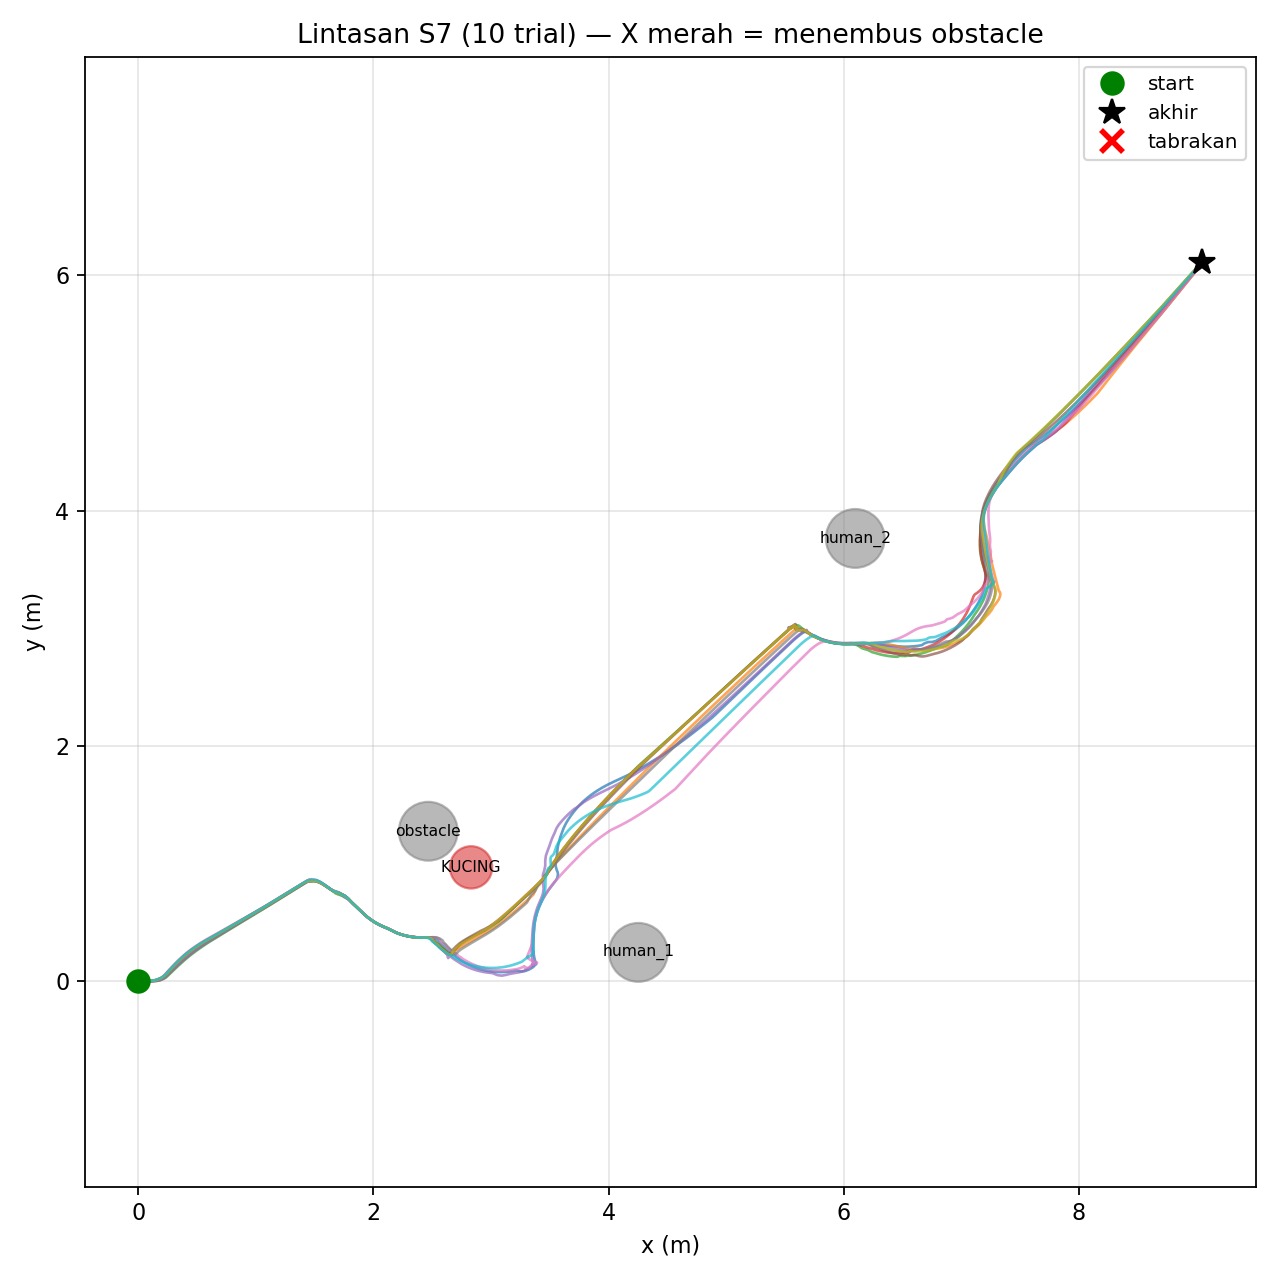
\includegraphics[width=\textwidth]{gambar/4.6_traj_S7.png}
\caption{S7 (proposed)}
\end{subfigure}
\caption{Lintasan S3 (kiri) dan S7 (kanan), lingkungan dengan \textit{obstacle}
statis majemuk dan kucing pada area \textit{blind-spot}. Tanda X pada panel
kiri merupakan deteksi jarak sesaat dari skrip visualisasi dan tidak
mencerminkan \texttt{collision\_count} resmi pada Subbab~\ref{sec:keberhasilan_tabrakan}
(lihat audit pada teks).}
\label{fig:traj_s3s7}
\end{figure}

Pada pasangan S3/S7 (Gambar~\ref{fig:traj_s3s7}), pola yang teramati justru
berlawanan dengan ekspektasi sederhana bahwa metode usulan selalu lebih
mulus. Kesepuluh \textit{trial baseline} (S3) hampir berimpit sempurna,
selalu mengambil rute yang sama persis di dekat kucing, sedangkan kesepuluh
\textit{trial proposed method} (S7) menyebar lebih lebar, beberapa
mengambil rute yang nyata berbeda di sekitar kelompok \textit{obstacle}.
Setiap lintasan individual pada S7 tetap berbentuk kurva yang halus, tidak
menunjukkan pola zig-zag tajam seperti pada S2; perbedaan utamanya adalah
\textit{konsistensi antar-trial}, bukan kehalusan dalam satu lintasan.
Temuan ini konsisten dengan standar deviasi minimum clearance pada
Subbab~\ref{sec:analisis_keselamatan}: 0,074~m pada S7 dibandingkan hanya
0,001~m pada S3, yang menggambarkan rentang variasi respons yang jauh lebih
lebar pada konfigurasi fuzzy ketika berhadapan dengan kombinasi \textit{blind-spot}
dan \textit{obstacle} majemuk.

\begin{figure}[H]
\centering
\begin{subfigure}[t]{0.48\textwidth}
\centering
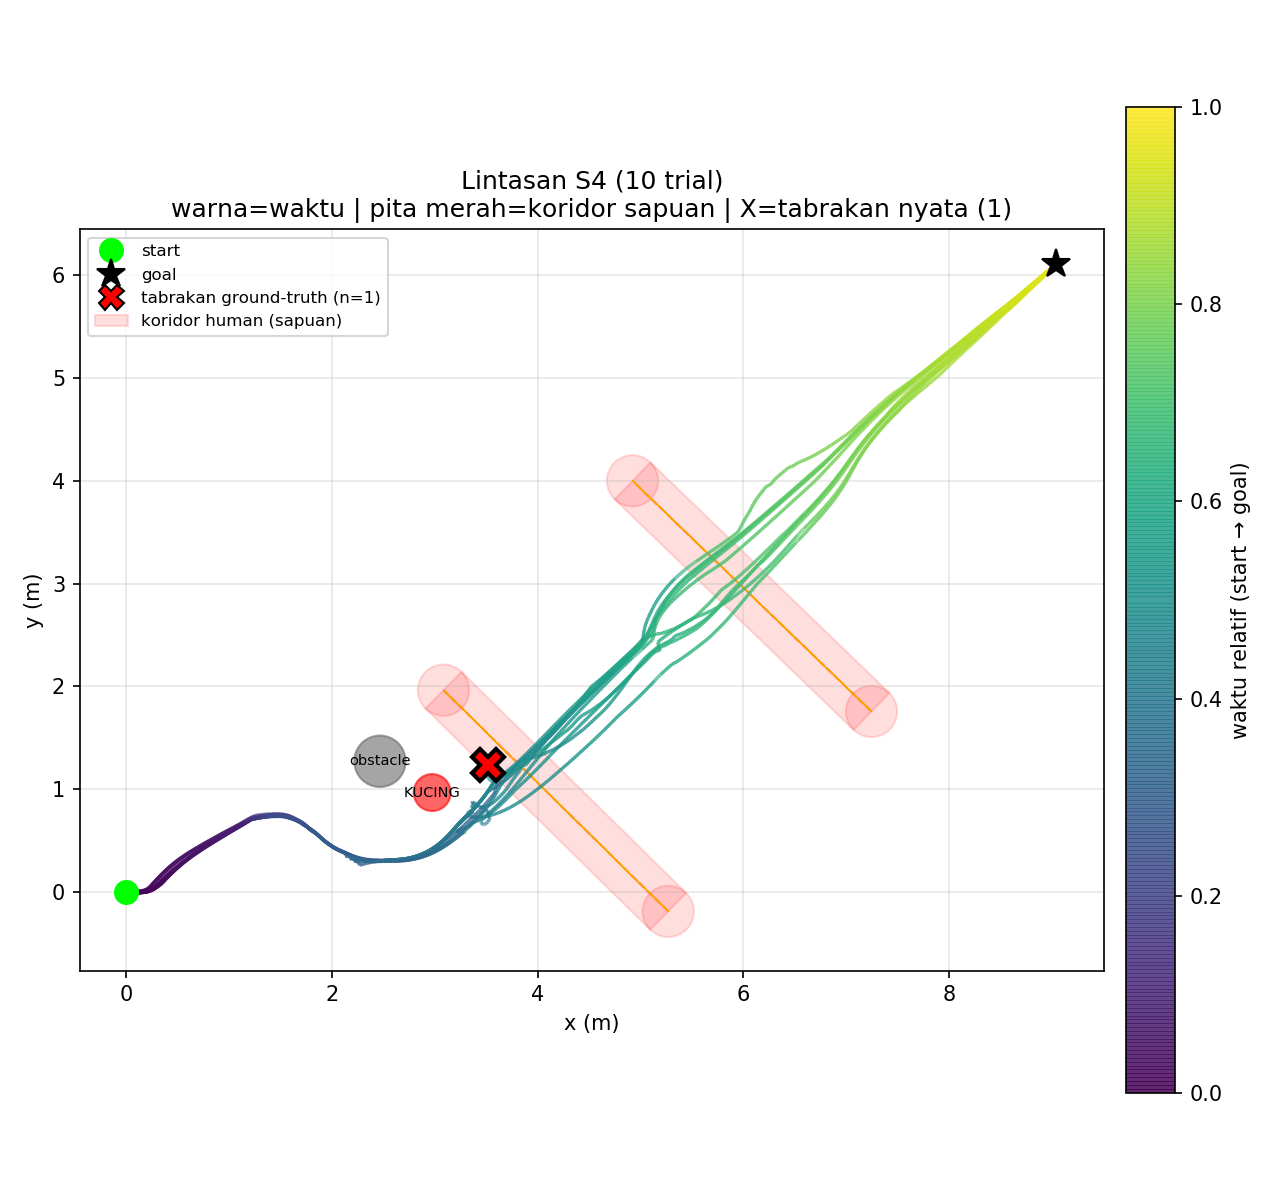
\includegraphics[width=\textwidth]{gambar/4.6_traj_S4_dynamic.png}
\caption{S4 (baseline)}
\end{subfigure}
\hfill
\begin{subfigure}[t]{0.48\textwidth}
\centering
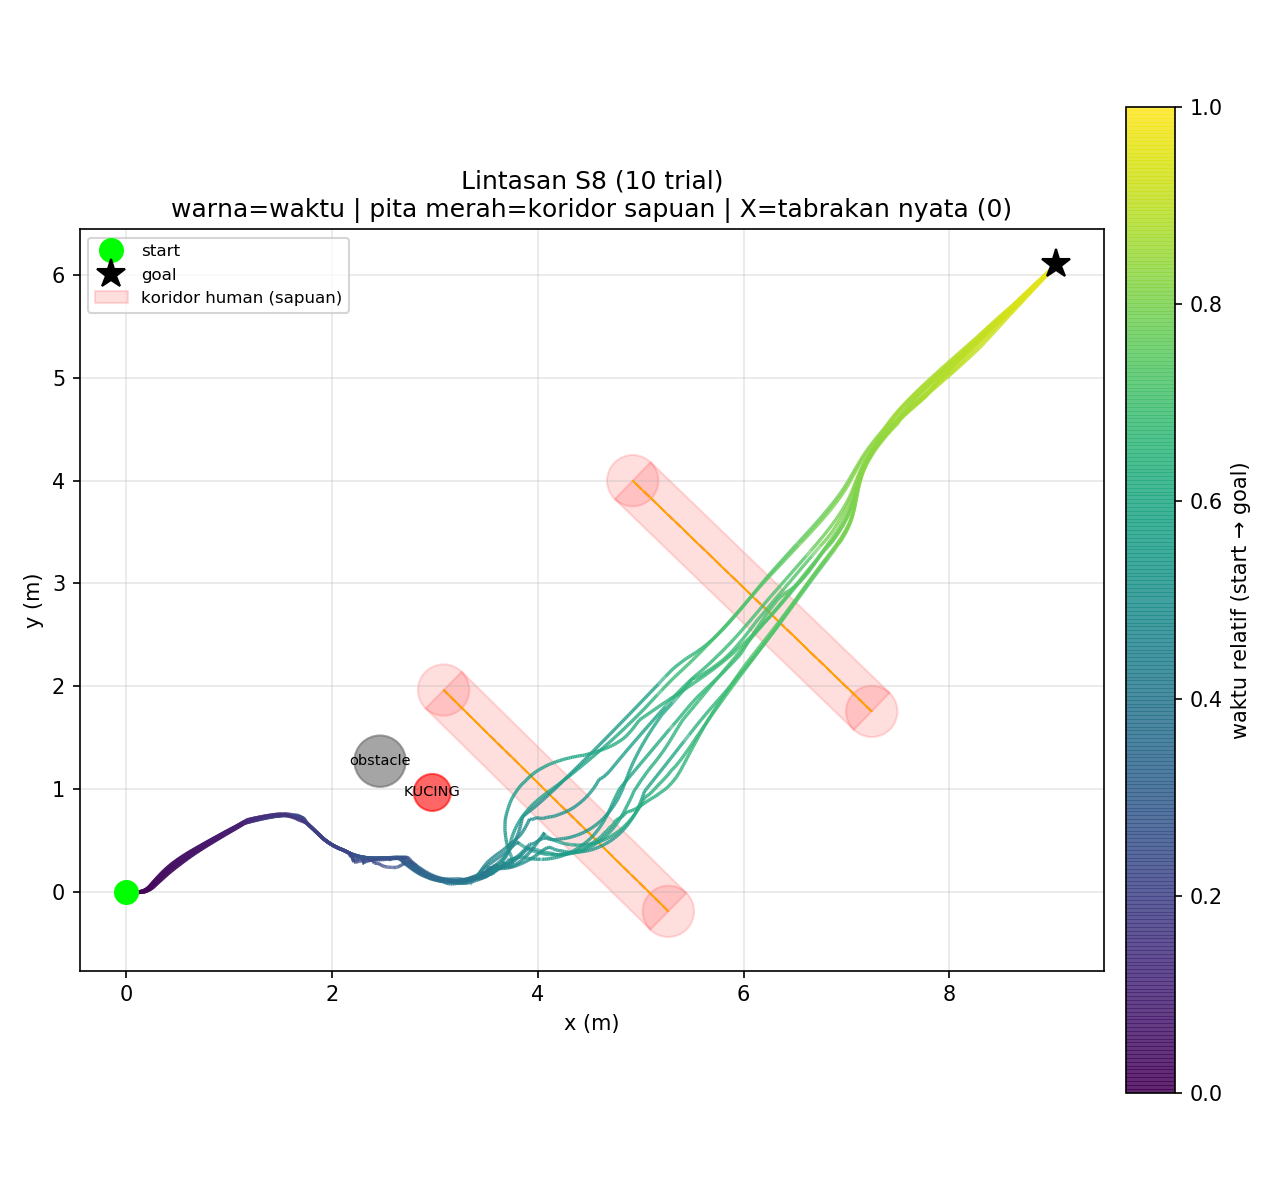
\includegraphics[width=\textwidth]{gambar/4.6_traj_S8_dynamic.png}
\caption{S8 (proposed)}
\end{subfigure}
\caption{Lintasan S4 (kiri) dan S8 (kanan) versi koridor-dinamis, lingkungan
dengan \textit{obstacle} dinamis. Pita merah menunjukkan koridor sapuan
\textit{obstacle\_human}; tanda X merupakan tabrakan \textit{ground-truth}
aktual sesuai \texttt{results.csv}.}
\label{fig:traj_s4s8}
\end{figure}

Pada pasangan S4/S8 (Gambar~\ref{fig:traj_s4s8}), \textit{trial baseline}
(S4) menunjukkan penyebaran rute yang nyata setelah melewati area kucing,
beberapa \textit{trial} mengambil jalur yang jauh berbeda saat mendekati
\textit{goal}, termasuk satu \textit{trial} yang berakhir pada tabrakan
\textit{ground-truth} (ditandai X) sebagaimana telah dibahas pada
Subbab~\ref{sec:keberhasilan_tabrakan}. Sebaliknya, kesepuluh \textit{trial
proposed method} (S8) tampak lebih konsisten satu sama lain meskipun
melintasi koridor sapuan \textit{obstacle} yang sama. Pada metrik kecepatan
angular rata-rata, kedua konfigurasi pada pasangan ini tidak menunjukkan
perbedaan yang berarti (dibahas pada bagian statistik berikut), sehingga
perbedaan yang teramati di sini lebih tepat digambarkan sebagai perbedaan
konsistensi antar-\textit{trial}, bukan perbedaan kehalusan gerak rata-rata.

\subsection{Analisis Statistik dan Effect Size}

Perbedaan kecepatan angular antara kedua konfigurasi diuji menggunakan uji
Mann-Whitney U, mengikuti metode yang sama seperti subbab-subbab sebelumnya.
Metrik \texttt{recovery\_count} tidak diuji secara statistik karena
tercatat 0 pada keseluruhan 80 \textit{trial} tanpa terkecuali, sehingga
tidak memiliki variansi yang dapat dibandingkan; nilai ini tetap dilaporkan
sebagai indikator bahwa mekanisme \textit{recovery} bawaan \texttt{move\_base}
tidak pernah terpicu pada kedua konfigurasi, mengindikasikan stabilitas
navigasi tingkat tinggi secara umum.

\begin{table}[H]
\centering
\caption{Hasil uji Mann-Whitney U untuk kecepatan angular pada keempat
pasangan skenario ($\alpha=0,05$).}
\label{tab:angvel_mwu}
\begin{tabular}{lcccc}
\toprule
\textbf{Pasangan} & \textbf{$U$} & \textbf{$p$} & \textbf{Signifikan} \\
\midrule
S1--S5 & 100 & 0,0002 & *** \\
S2--S6 & 100 & 0,0002 & *** \\
S3--S7 & 6   & 0,0009 & *** \\
S4--S8 & 38  & 0,4055 & ns  \\
\bottomrule
\end{tabular}
\end{table}

\begin{table}[H]
\centering
\caption{Effect size (\textit{rank-biserial correlation}) untuk kecepatan
angular pada keempat pasangan skenario.}
\label{tab:angvel_effect_size}
\begin{tabular}{lcc}
\toprule
\textbf{Pasangan} & \textbf{Effect Size ($r$)} & \textbf{Interpretasi} \\
\midrule
S1--S5 & -1,00 & Besar \\
S2--S6 & -1,00 & Besar \\
S3--S7 & +0,88 & Besar \\
S4--S8 & +0,23 & Kecil \\
\bottomrule
\end{tabular}
\end{table}

Tabel~\ref{tab:angvel_mwu} dan Tabel~\ref{tab:angvel_effect_size}
menunjukkan bahwa konfigurasi \textit{proposed method} menghasilkan
kecepatan angular yang signifikan lebih rendah pada S1/S5 dan S2/S6
(\textit{effect size} besar), namun signifikan lebih \textit{tinggi} pada
S3/S7 (\textit{effect size} besar juga, namun berlawanan arah), sedangkan
pada S4/S8 tidak terdapat perbedaan yang signifikan (\textit{effect size}
kecil). Pola ini menegaskan bahwa kontribusi fuzzy terhadap kehalusan gerak,
diukur dari kecepatan angular rata-rata, tidak seragam pada seluruh kondisi
lingkungan.

\subsection{Hubungan dengan APF dan Fuzzy}

APF secara teoritis rentan terhadap osilasi di sekitar \textit{obstacle}
pada \textit{local minima}, dan mekanisme deteksi osilasi pada
Persamaan~\ref{eq:osc_detect} telah dirancang sebagai mitigasi dasar yang
berlaku pada kedua konfigurasi. Adaptasi fuzzy berpotensi memodulasi
respons repulsif secara lebih halus melalui penyesuaian penguatan dan
kecepatan, dan hasil pada S1/S5 serta S2/S6 konsisten dengan potensi
tersebut. Namun, hasil pada S3/S7 menunjukkan bahwa modulasi ini tidak
selalu menghasilkan kecepatan angular yang lebih rendah, kecepatan angular
proposed method pada pasangan ini justru lebih tinggi, kemungkinan karena
sistem melakukan lebih banyak penyesuaian arah saat menavigasi kombinasi
\textit{obstacle} majemuk dan area \textit{blind-spot} secara lebih
eksploratif. Dengan demikian, data pada penelitian ini tidak mendukung
klaim bahwa adaptasi fuzzy sepenuhnya menghilangkan osilasi atau secara
seragam menghasilkan gerakan yang lebih halus pada seluruh kondisi; yang
dapat disimpulkan secara valid adalah bahwa kontribusinya terhadap
kehalusan gerak bersifat tergantung kondisi lingkungan.

Beberapa keterbatasan perlu dicatat dalam membaca hasil ini. Pertama,
resolusi \textit{sampling} pada \texttt{experiment\_logger.py} dapat
memengaruhi kehalusan kurva lintasan yang teramati secara visual, sehingga
detail osilasi frekuensi tinggi yang berada di bawah resolusi tersebut
tidak tertangkap. Kedua, evaluasi visual terhadap trajektori bersifat
parsial dan melibatkan penilaian kualitatif, yang meskipun didukung data
kuantitatif pendukung, tetap berpotensi bias subjektif. Ketiga, seluruh
hasil belum divalidasi pada robot fisik, sehingga karakteristik osilasi
pada permukaan dan aktuator nyata belum dapat dipastikan sama dengan hasil
simulasi ini.

Setelah mengevaluasi kualitas gerak pada subbab ini, analisis selanjutnya
membahas hasil uji statistik secara terintegrasi untuk seluruh metrik utama
penelitian. Subbab berikutnya merangkum temuan tersebut pada Subbab 4.7.